\section{Function Component} \label{sc:function_component}
Having added new attributes, classes, and structures to the class diagram through the model component, the functions from the function list can be implemented as well. Some of these functions should be implemented in the classes directly, others should be placed in the function component. The following section contains additions to the original function list, the arguments for these additions, decisions about implementations of these, and the final function component design.
\par
Throughout this sections, only the most essential functionalities will be described. There are smaller classes that have responsibilities less essential to the core functionality of the system, which will not be described.

\subsection{Additions to the function list}
The function list (see \autoref{tab:functions} on page \pageref{tab:functions}) has been constructed based on the original class diagram (see \autoref{fig:FirstPDClassDiagram}), but does not accommodate the new additions from the model component. To support the new classes, the following functions have been added:

\begin{table}[H]
\centering
    \begin{tabular}{|c|l|l|l|}
        \hline
        \textbf{Nr.} & \textbf{Function name} & \textbf{Complexity} & \textbf{Function type}\\
        \hline
        1 & Get asset by id & Simple & Read\\
        \hline
        2 & Get department by id & Simple & Read\\
        \hline
        3 & Get tag by id & Simple & Read\\
        \hline
        4 & Search for tag & Medium & Compute/Read\\
        \hline
        5 & Add field to asset/tag & Medium & Update\\
        \hline
        6 & Update tag information & Simple & Update\\
        \hline
        7 & Update department information & Simple & Update\\
        \hline
        8 & Tag created & Simple & Update\\
        \hline
        9 & Tag deleted & Simple & Update\\
        \hline
        10 & Tag attached & Medium & Update\\
        \hline
        11 & Tag detached & Medium & Update\\
        \hline
    \end{tabular}
\end{table}

Functions 1-3 are added to read the objects from the model to the application domain. The \textit{Get asset by id} function replaces the \textit{View asset} function, as they both fetch the object.
\par
Function 4 makes it possible to search for a tag, in the same way as it is possible to search for an asset.
\par
Function 5 makes it possible to add a field to an asset or a tag.
\par
Functions 6 and 7 handle the updating of the tags and departments in the system. This lets the user maintain the tags and departments, as they change name or, for the tags, need more functionality.

\subsection{Design}
The following includes examinations of the functions and design decisions about how they should be incorporated in the component design. To better separate the responsibility of the different classes, the \textit{Asset}, \textit{Comment}, \textit{Department}, \textit{Field}, \textit{User}, and \textit{Tag} classes have been implemented as simple data classes. This means that they will simply store data and only perform operations related to interpreting the data of the model.

\subsubsection{Maintaining the model}
All the \textit{add}, \textit{remove}, \textit{update}, and \textit{get by id} functions are used by an employee with admin status. These functions should be handled similarly for assets, departments, users, and tags, and therefore they will all be grouped into a strategy \citep{OOAD}. A thorough look at these functions and the structure will show that this pattern is actually a repository pattern \citep{RepositoryPatternDescription}.
\par
An intuitive name of the class describing the overall strategy is \textit{Repository}. The class is abstract, as every class acting as a concrete strategy will inherit the functions from the \textit{Repository}. The concrete classes handle the assets, departments, users and tags respectively and have been named: \textit{AssetRepository}, \textit{DepartmentRepository}, \textit{UserRepository}, and \textit{TagRepository}. These control the maintenance of the data for their designated classes in the model.
\par
As mentioned, these concrete classes have operations for adding, removing, and updating, which all take an object of the designated class, and an operation for getting an object by id. This structure has been placed in the function component, as it does not belong to a specific class in the model component. 
\begin{figure}[H]
    \centering
    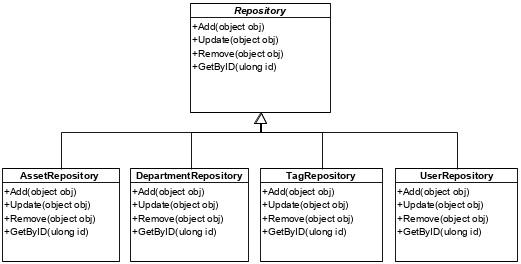
\includegraphics[width=0.85\textwidth]{figures/FunctionComponent/Repository_pattern.png}
    \caption{The repository pattern for maintaining data in the model}
    \label{fig:RepositoryPattern}
\end{figure}

\subsubsection{Attach and detach tag}
The operations of attaching or detaching a tag to or from an asset is called by an admin and involves the \textit{Tag} and \textit{Asset} classes. The functions create or delete an instance of the \textit{Asset-tag relation} class containing the involved asset and tag. The operations should be added to a class in the function component, as the admin does not carry out the operations.
\par
The operations have been placed in the \textit{AssetRepository} class, as the asset is responsible for maintaining the connections to its attached tags. Placing them directly on the \textit{Asset} class, however, would give the class responsibility of an operation in which it participates solely as an object. The operations have been named \textit{AttachTags} and \textit{DetachTags}. Both operations take two parameters, an asset, and a list of tags to be attached to the asset.

\begin{figure}[H]
    \centering
    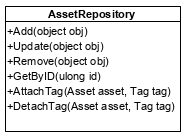
\includegraphics[width=0.3\textwidth]{figures/FunctionComponent/AttachTag.png}
    \caption{The \textit{AssetRepository} class with the \textit{AttachTag} and \textit{DetachTag} operations}
    \label{fig:AttachDetachTag}
\end{figure}

\subsubsection{Search for asset or tag}
The \textit{search for asset} function lets the user search through the assets in the system and returns the assets that comply with the search query. Multiple assets are handled and therefore it would not be intuitive to add it as an operation on the asset class. It is called by the user, but the user is not responsible for searching through the assets, so the function has been placed as an operation in the function component.
\par
The function \textit{search for tag} goes through the same process and both functions have the same structure. The search is carried out on the elements in the database and therefore they fit well into the specialized classes of the \textit{Repository} class.

\begin{figure}[H]
    \centering
    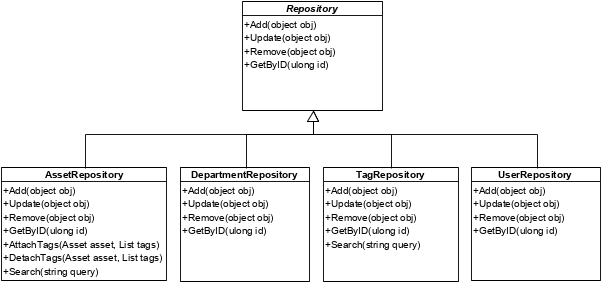
\includegraphics[width=0.92\textwidth]{figures/FunctionComponent/Repository_pattern_with_search.png}
    \caption{The repository pattern with the search operations for assets and tags}
    \label{fig:RepositoryPatternWithSearch}
\end{figure}

\subsubsection{Comment asset}
Commenting on an asset adds a comment to the asset. It is desired that the comments can be retrieved and shown without retrieving the entire asset, to which it belongs. The reason for this is that the newest comments are to be shown on the home page of all admins, to give an overview of the latest changes and problems. Therefore the comments will not be placed directly on the asset, but will be stored separately and contain a relation to the asset. Because of this, the comment will need the functions \textit{add}, \textit{remove}, \textit{update}, and \textit{get by id} and can therefore be seen as another specialized class of the \textit{Repository} class.

\begin{figure}[H]
    \centering
    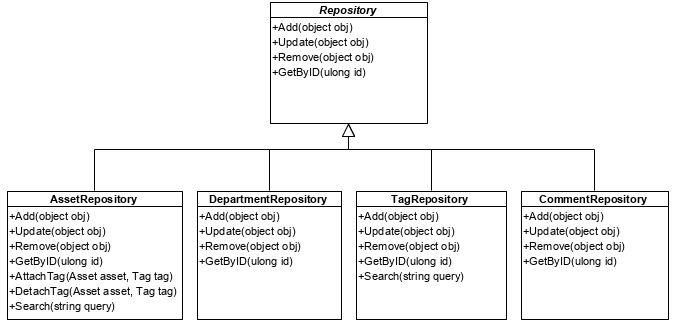
\includegraphics[width=1\textwidth]{figures/FunctionComponent/CommentRepository.png}
    \caption{The repository pattern with the \textit{CommentRepository}}
    \label{fig:RepositoryPatternWithCommentRepository}
\end{figure}

\subsubsection{Authenticate user \& Check access level}
As mentioned in \autoref{sc:model_component}, the \textit{Employee} and \textit{Admin} classes are used to differentiate between users with and without administrative access to the system. This should not be handled by the models themselves, which has let to the creation of a new class in the function component called \textit{Session}. This, in combination with the addition of the \textit{Tag} class, makes the \textit{Admin} and \textit{Employee} classes obsolete.
\par
The operations for authenticating and checking access level of users have been named \textit{Authenticated} and \textit{IsAdmin}. \\
The \textit{Session} class also contains the attributes \textit{Username} and \textit{Domain}, to make sure that the information about the employee currently logged in is available to the system.

\begin{figure}[H]
    \centering
    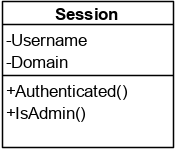
\includegraphics[width=0.22\textwidth]{figures/FunctionComponent/Session.png}
    \caption{The \textit{Session} class}
    \label{fig:session_class}
\end{figure}

% \subsubsection{Export report}
% The operation has been placed in a class in the function component named \textit{ExportHandler}.
% \begin{figure}[H]
%     \centering
%     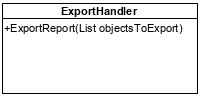
\includegraphics[width=0.4\textwidth]{figures/FunctionComponent/ExportHandler.png}
%     \caption{The \textit{ExportHandler} class}
%     \label{fig:ExportHandler}
% \end{figure}

\subsubsection{Updating data classes}
To ensure that the data in the data classes is handled correctly, controllers have been introduced between the data classes and the related classes in the function component. This ensures that the data is correctly handled and valid, before saving it to the data classes.
\par
The controllers handle communication with classes that either need information from the data classes or change some of the information. They also handle communication with the repositories. This makes it possible to call methods in a controller, which then formats the data class and sends them to the associated repository.
\par
The controllers differ in functionality and therefore does not build on a generalized controller. Two controllers have been depicted in the picture below (see \autoref{fig:AssetControllerAndAssetListControllerClasses}).

\begin{figure}[H]
    \centering
    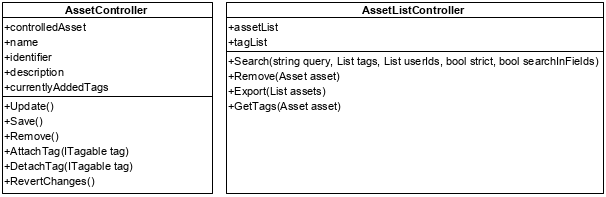
\includegraphics[width=0.95\textwidth]{figures/FunctionComponent/AssetControllerAndAssetListController.png}
    \caption{The \textit{AssetController} and \textit{AssetListController} classes}
    \label{fig:AssetControllerAndAssetListControllerClasses}
\end{figure}

The \textit{AssetController} handles only one asset and gives the dependent classes access to the operation they need, in context of reading and updating the asset. One of these is the \textit{Save} operation, which simply calls the \textit{AssetRepository} with the controlled asset. This way, the surrounding classes do not need any knowledge of the repository doing the operation  save the asset.
\par
The \textit{AssetListController} contains a list of assets and makes it possible for the dependent classes to interact with the list, such as searching through the list and removing an asset from the list. As mentioned above, the controller makes it possible for the dependent classes to ignore the existence of certain classes, such as the repositories.

\subsubsection{Add or remove field to asset or tag}
Adding a field to either an asset or a tag will create a field directly on the asset or tag. The fields do not have their separate place in the system, as they are not relevant without either the asset or the tag, to which they belong. Therefore the function has been implemented in the function component as an operation in an abstract class called \textit{FieldListController}.
\par
The class defines operations such as adding or removing a field to or from a data class (see \autoref{fig:FieldListController}).

\begin{figure}[H]
    \centering
    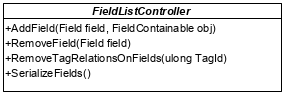
\includegraphics[width=0.5\textwidth]{figures/FunctionComponent/FieldListController.png}
    \caption{The \textit{FieldListController} class}
    \label{fig:FieldListController}
\end{figure}

\subsubsection{Additional classes}
Other classes have been added but are not included in the previous description, as they are not part of the core functionality. The functionality of these classes include logging changes, which is handled by the \textit{Logger} class and saved using the \textit{LogRepository} class. Others are the \textit{Exporter} class handling exporting items from the system, the \textit{FileEncryption} class that secures the application database credentials, and the \textit{UserImporter} that imports users to the system, from a CSV file. The mentioned classes are not implementing core functionality and are therefore not shown in the component diagram either (see \autoref{fig:FunctionComponent}).

\subsection{Function component diagram}
Based on the decisions made in this section, the function component has been constructed and is illustrated in \autoref{fig:FunctionComponent}.

\begin{figure}[H]
    \centering
    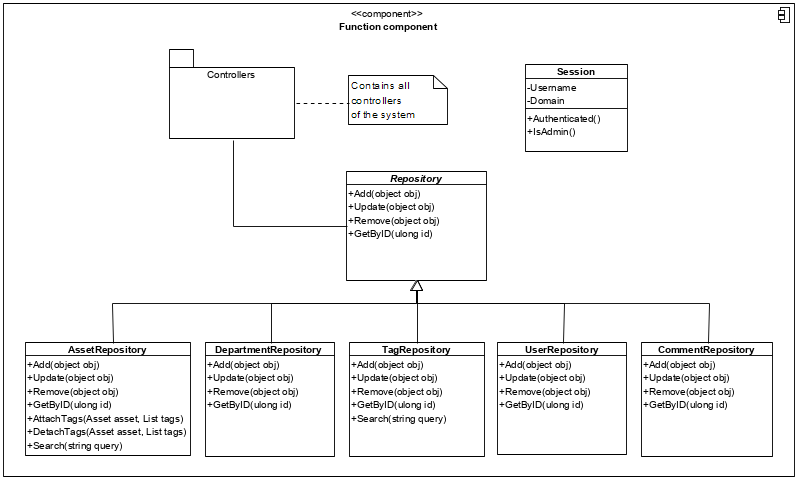
\includegraphics[width=\textwidth]{figures/FunctionComponent/FunctionComponent.png}
    \caption{Illustration of the function component of the system}
    \label{fig:FunctionComponent}
\end{figure}

The overall behaviour of the system is pretty simple, as it only has the state \textit{active}. Therefore, a diagram of this behaviour is trivial and has not been included here.
\newpage